\subsection{Management and Organization}
As a start up company progresses, resources and workforce increase. To ensure responsibilities and daily tasks a hierarchy can be structured within the company. Ground rules have to be set early on to avoid discussions and arguments throughout the process. Below is a description of the organisational structure, ownership, key activities and resources.

\subsubsection{Legal Structure and Ownership}
The rights to this concept are distributed equally amongst the group members. 
This was decided in the beginning of the project and is written in the group contract.
Since the group consists of students, the project will require funding to become a reality. No one is interested in being personally liable for the debt should the company go bankrupt. 
For this reason creating an ApS would be a good option. 
This requires at least 50.000 kr. of value (can be values of objects too) to settle. The risk of doing it this way is that the investors will probably force the group members to sign for a personal liable agreement. 
Ownership is likely to change as investors will most likely require a share of the company as compensation for their investment.

\subsubsection{Management}
The management structure is based on a conclusion drawn from the Belbin group result. It is based on the requirements of the different titles within the company. For instance, we felt that the CEO would require a strong represent who has a great overview (Acts as a coordinator), a talent for communication (Resource Investigator) and the drive of a shaper. Within these three fields, a score was created based on the individual Belbin results, which lead to choosing David as the CEO. 
The same procedure was followed when assigning candidates for the other posts. 
% \begin{itemize}
% \item CEO, David
% \item CTO, Xabier
% \item CFO, Casper
% \end{itemize}

Nikolaj, Thomas, Simon and Kirstine are chosen as the implementers as they are best suited for programming and doing the assembly of the product.
It is obvious from figure \ref{management_structure} that our management structure is heavily based on development and thus the chief technical officer is a very key role in this type of company.

\begin{figure}[ht]
\centering
    \tikzstyle{mp} = [font=\footnotesize, draw, rectangle, fill=blue!10, text=black, text width = 3.7em, minimum height =4.1em, text centered]
  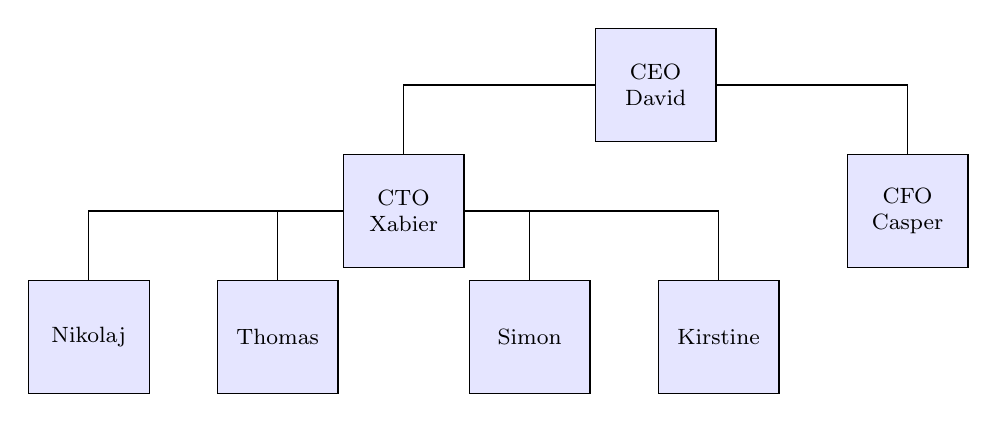
\begin{tikzpicture}[scale=0.8]
  \draw (0,0)
  node[mp] (ceo)                     {CEO\\David} 
  (ceo) -| ++(-4,-2) node[mp] (cto)  {CTO\\Xabier} 
  (ceo) -| ++( 4,-2) node[mp] (cfo)  {CFO\\Casper}
  
  (cto) -| ++(-5,-2) node[mp] (impA) {Nikolaj}
  (cto) -| ++(-2,-2) node[mp] (impb) {Thomas}
  (cto) -| ++( 2,-2) node[mp] (impc) {Simon}
  (cto) -| ++( 5,-2) node[mp] (impd) {Kirstine}
  ;  
  \end{tikzpicture}
  \caption{Management structure of Interflex}
  \label{management_structure}
\end{figure}


\subsubsection{Board and Advisors}
As usual, the leaders of a company will be sitting within the board, but different partners would also play a big role. 
If a company decides to buy our product, for using it in their own solutions, they could have an interest in having a member in our board because they may wish to influence the development in a certain direction. 
They are the ones who sell to the end users and if they do not have any sales, our company makes no profit either, so having them influence the product and development could benefit both of companies. 
It could be interesting to have other partners within the board, especially some within the technological field, robot- and software wise.
One of the most valuable advisors to have would be a person with experience within innovation and technology, who also has experience with a start up company. 

\subsubsection{Key Partners}
The strategy of the company relies on having distributors for the regions where we wish to do business, therefore it is essential to have partnerships with these companies. They are not the final customer of our company, but a link to them. This is where the main revenue streams are going to be created.
For instance, Valk Welding would be an optimal partner within the Danish market, since they are able to reach the final customers within Denmark. It is our goal to reach distributors like Valk Welding within the european market.
Another sort of interesting partners is one of the majors of the market. This could be Migatronic, Valk Welding, Universal Robots or any other sort of major company within the field of welding technology, who already exist on the market. The reason for this is that they could be interested in the technology our product offers and that they would like to integrate it within their range of products. This situation would usually lead to them investing in our company and putting a limit to which companies we are allowed to collaborate with.

\subsubsection{Key Activities}
Throughout the course of the project there are a few well defined activities that we must cover for the project to be successful. These activities are described here:

\begin{itemize}
	\item \textbf{Funding		:} Initially funding must be in place. The development relies on the team being able to invest in hardware for testing software. 
	\item \textbf{Development	:} When funding is in place the development process can begin. Initially software will be developed for controlling the individual parts of the tool, allowing for testing of the parts so that suitable parts can be chosen for the tool. Once the housing has been designed and manufactured, work can be made towards the initial prototype.
	\item \textbf{Distributers	:} During the development process work will be done to find suitable partners that are capable of handling the distribution of our tool.
	\item \textbf{Production	:} When a working prototype has been developed, production can begin. A suitable work space where the assembly of the product can be done must be found. The assembly will initially be done by members of the team to save money on labour costs. 
	\item \textbf{Maintenance	:} After the product has been distributed and initial development is complete, it is necessary to provide customers with assistance. Any problems regarding the software will be fixed by regular updates. During this phase we will also attempt to expand compatability of the tool to fit a larger range of robots.
\end{itemize} 

A further description of these activities as well as the goals that each activity encompass can be found in section \ref{sec:actionDevelopmentPlan}
\subsubsection{Key Resources}
The key resources are the assets to the company that are necessary for creating value for the customer. These will support the company and make it sustainable.
To summarize the primary key resources to the company:
\begin{itemize}
\item Injection of funds
\item Accommodations for office and development usage
\item Patenting the product
\end{itemize}
